Hva kan man bruke dioder til?

\subsubsection{Powersupply}
En PSU brukes i alle DC enheter som henter strøm fra AC nettet.
F.eks. en datamaskin.
Vekselstrømmen fra strømnettet må konverteres til
et stabilt DC signal før det kan brukes.
\\\\
AC signalet kjøres først gjennom en likeretter,
for å bli kvitt negativ spenning.
Deretter gjennom et elektronisk filter,
som fjerner mesteparten av spenningsvariasjonene.
Spenningen har nå små variasjoner og kalles ripple.
Noen enheter trenger et finere signal enn dette og
signalet kjøres gjennom en spenningsregulator.
\\\\
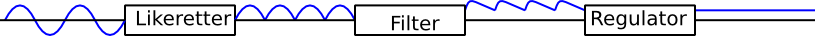
\includegraphics[width=\textwidth]{./img/psu}



\subsubsection{Likeretter}
I PSUen sitter en likeretter.
Her er mer detalj om hvordan den fungerer.

\paragraph{Halvbølge} \mbox{} \\
I en halvbølge-likeretter blir enten den positive eller den negative
halvdelen av AC signalet sluppet igjennom.
\\\\
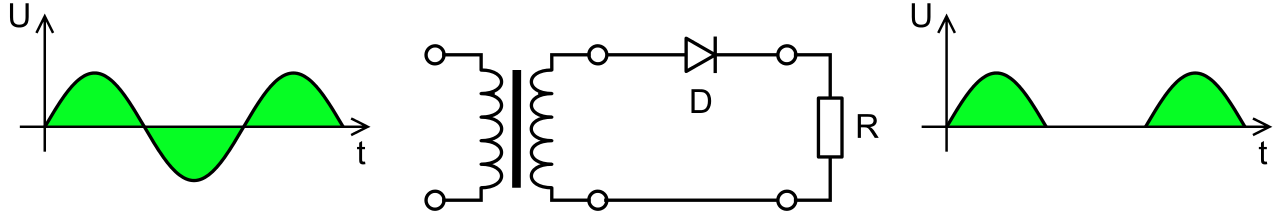
\includegraphics[width=\textwidth]{./img/halvbolge}

\paragraph{Helbølge} \mbox{} \\
Diodene slipper igjennom strøm i bare én retning.
\\\\
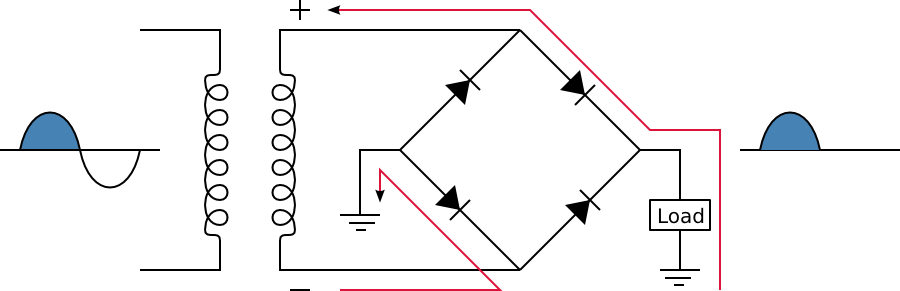
\includegraphics[width=\textwidth]{./img/likeretter}
\\\\
Når spenningen reverseres, slipper de andre diodene strøm igjennom.
\\\\
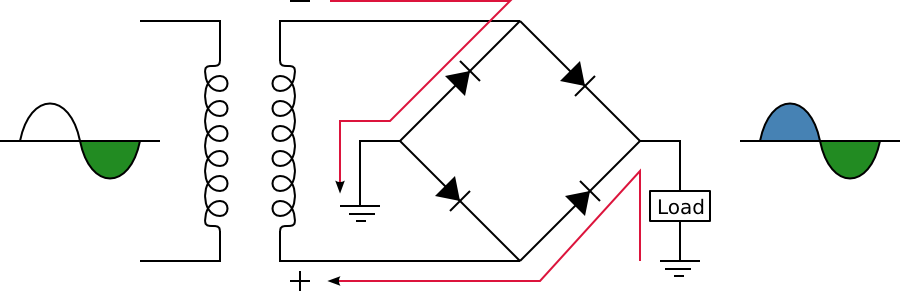
\includegraphics[width=\textwidth]{./img/likeretter-rev}
